\documentclass[a4paper,landscape]{article}


\usepackage{tikz}
 \usetikzlibrary{arrows}
\usetikzlibrary{fit,positioning}



\begin{document}

%\centering
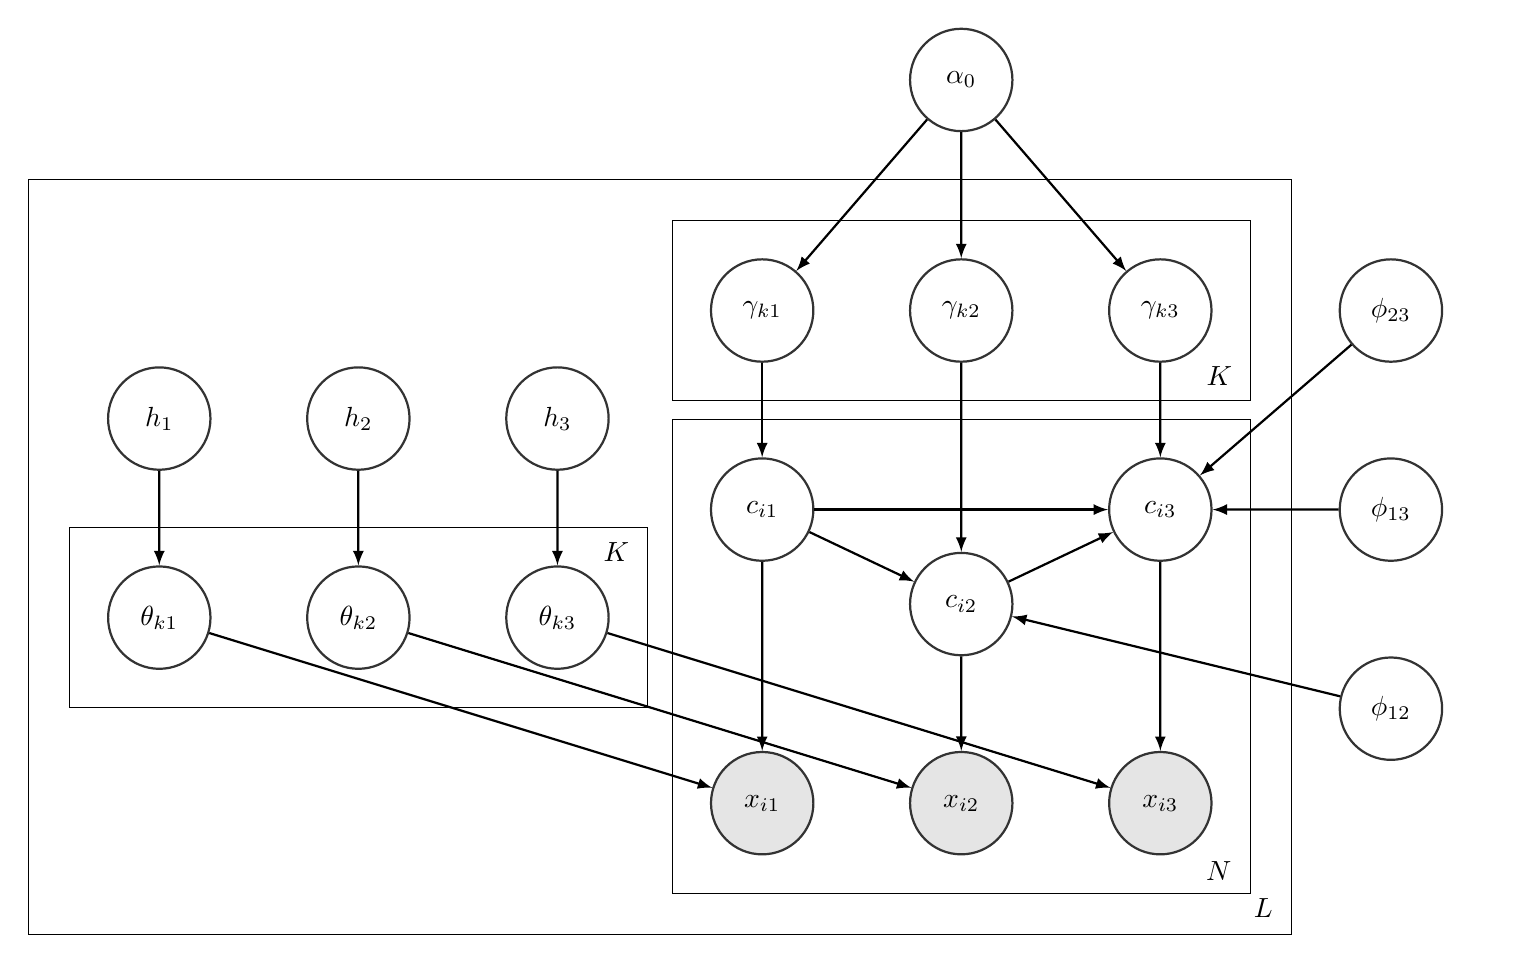
\begin{tikzpicture}[scale=.65, auto,>=latex']
\tikzstyle{main}=[circle, minimum size = 13mm, thick, draw =black!80, node distance = 12mm]
\tikzstyle{connect}=[-latex, thick]
\tikzstyle{box}=[rectangle, draw=black!100]

\node[main] (pi1) {$\gamma_{k1}$ };
 \node[main] (pi2) [right=of pi1] {$\gamma_{k2}$ };
 \node[main] (pi3) [right=of pi2] {$\gamma_{k3}$ };
 
 \node[main] (ci1) [below=of pi1] {$c_{i1}$};
 \node[main, node distance = 24mm] (ci2) [below=of pi2] {$c_{i2}$};
 \node[main] (ci3) [below=of pi3] {$c_{i3}$};
 
 \node[main, node distance = 16mm] (a) [above=of pi2] {$\alpha_0$ };

 \node[main, fill = black!10] (xi2) [below=of ci2] {$x_{i2}$}; 
 \node[main, fill = black!10] (xi1) [left=of xi2] {$x_{i1}$};
 \node[main, fill = black!10] (xi3) [right=of xi2] {$x_{i3}$};

 \node[main]  at (-4, -6) (theta3) {$\theta_{k3}$}; 
 \node[main] (theta2) [left=of theta3] {$\theta_{k2}$};
 \node[main] (theta1) [left=of theta2] {$\theta_{k1}$};

 
 \node[main] (h1) [above=of theta1] {$h_1$};
 \node[main] (h2) [above=of theta2] {$h_2$};
 \node[main] (h3) [above=of theta3] {$h_3$};

 \node[main, minimum size=1.3cm, node distance = 16mm] (phi13) [right=of ci3] {$\phi_{13}$}; 
 \node[main, minimum size=1.3cm] (phi12) [below=of phi13] {$\phi_{12}$};
 \node[main, minimum size=1.3cm] (phi23) [above=of phi13] {$\phi_{23}$};

 \node[rectangle, inner sep=-0.5mm, fit= (ci1) (ci2) (ci3) (xi1) (xi2) (xi3),label=below right:$N$, xshift=5mm, yshift=0mm] {};
 \node[rectangle, inner sep=4.8mm,draw=black!100, fit= (ci1) (ci2) (ci3) (xi1) (xi2) (xi3)] {};
 
% \node[rectangle, inner sep=-0.8mm, fit= (theta1) (theta2) (theta3) (pi1) (pi2) (pi3) ,label=above right:$K$, xshift=63mm] {};
% \node[rectangle, inner sep=4.8mm, draw=black! 100, fit= (theta1) (theta2) (theta3) (pi1) (pi2) (pi3)] {};

 \node[rectangle, inner sep=-0.8mm, fit= (theta1) (theta2) (theta3) ,label=above right:$K$, xshift=24mm] {};
 \node[rectangle, inner sep=4.8mm, draw=black! 100, fit= (theta1) (theta2) (theta3)] {};

 \node[rectangle, inner sep=-0.8mm, fit=  (pi1) (pi2) (pi3) ,label=below right:$K$, xshift=24mm] {};
 \node[rectangle, inner sep=4.8mm, draw=black! 100, fit= (pi1) (pi2) (pi3)] {};
 
 \node[rectangle, inner sep=-0.8mm, fit= (ci1) (ci2) (ci3) (xi1) (xi2) (xi3) (theta1) (theta2) (theta3) (pi1) (pi2) (pi3) (h1) (h2) (h3),label=below right:$L$, xshift=37mm, yshift=-5mm] {};
 \node[rectangle, inner sep=10.0mm, draw=black! 100, fit= (ci1) (ci2) (ci3) (xi1) (xi2) (xi3) (theta1) (theta2) (theta3) (pi1) (pi2) (pi3) (h1) (h2) (h3)] {};

 \path (pi1) edge [connect] (ci1)
    (pi2) edge [connect] (ci2)
    (pi3) edge [connect] (ci3)
    
		(ci1) edge [connect] (xi1)
		(ci2) edge [connect] (xi2)
		(ci3) edge [connect] (xi3)
		
		(ci1) edge [connect] (ci2)
		(ci1) edge [connect] (ci3)
		(ci2) edge [connect] (ci3)
		
		(theta1) edge [connect] (xi1)
		(theta2) edge [connect] (xi2)
		(theta3) edge [connect] (xi3)
		
		(h1) edge [connect] (theta1)
		(h2) edge [connect] (theta2)
		(h3) edge [connect] (theta3)
		
		(a) edge [connect] (pi1)
		(a) edge [connect] (pi2)
		(a) edge [connect] (pi3)
		
		(phi12) edge [connect] (ci2)
		(phi13) edge [connect] (ci3)
		(phi23) edge [connect] (ci3);

\end{tikzpicture}

\end{document}